\documentclass[10pt]{beamer}

\usepackage{appendixnumberbeamer}

\usepackage{booktabs}
\usepackage[scale=2]{ccicons}

\usepackage{pgfplots}
\usepgfplotslibrary{dateplot}

\usepackage{xspace}
\usepackage{../theme_style}
% \setbeameroption{show notes on second screen}

\title[Pervasive Computing]{Exam question five - Pervasive Computing}
\subtitle{Distributed and Pervasive Systems}
\date{June 03, 2022}
\author[M.H. Kristensen]{Morten Haahr Kristensen}
\def\studentid{201807664}
\institute{Department of Electrical and Computer Engineering - Aarhus University}
% Logo only on title page
\titlegraphic{
    
\includegraphics[width=12cm]{figs/aulogo_big.png}
}
\begin{document}

\maketitle

\begin{frame}{Outline}
  \setbeamertemplate{section in toc}[sections numbered]
  \tableofcontents[hideallsubsections]
\end{frame}

\section{Definitions}

\begin{frame}
  \frametitle{Pervasive Systems}
  Pervasive systems definition: \\
  \vspace*{-1.0em}
  \begin{quote}
    \textbf{Pervasive systems} are context-aware sensor-based \textbf{systems} which are \textbf{inspired} by \textbf{pervasive computing concepts}, methods and best practices, and which \textbf{relies} on \textbf{pervasive enabling technologies} to \textbf{achieve} a \textbf{calm}, \textbf{effective}, and \textbf{efficient} technology experience for their users. (Wagner 2022 \cite{wagnerPervasiveComputing2022})
  \end{quote}
  \note{
    Difference between pervasive computing and pervasive systems:\\
    Pervasive system is the architecture.\\
    Pervasive computing is the technique (how it is done).

    Calm technology: A technology that is designed to mainly occur in the user's periphery. The information only presents itself when needed and otherwise stays calmly on the user's periphery. 
    }
\end{frame}

\begin{frame}
  \frametitle{Smart stuff}
  Smart device
  \vspace*{2em}

  Smart environment
  \vspace*{2em}

  Smart space
  \vspace*{2em}

  Smart interaction
  
  \note{
    \footnotesize
    When talking about pervasive systems it is inevitable to run across the ''smart stuff''. We generally talk about three categories of smart x:\\
    Smart device: An electronic device that can connect, share and interact with a pervasive system. I.e. other smart devices. \\
    Smart environment: An environment that can acquire and apply knowledge about the environment and its users to improve their experience.\\
    Smart space: A smart space is a smaller area of a smart environment.\\
    A smart environment could be a hospital where the ventilation is automated, bed occupancy is tracked, and the nearest doctor is automatically called for if an emergency happens if he is not busy. A smart space in the hospital could be a specific room where the screen automatically opens the patients' journal when the nurse enters.\\
    Smart interaction: Dynamic organization and interaction between components to achieve shared goals. Can be internal or driven by external events.
  }

\end{frame}

\section{Background}

\begin{frame}
  \frametitle{Three (+ one) computing waves}
  \begin{figure}
    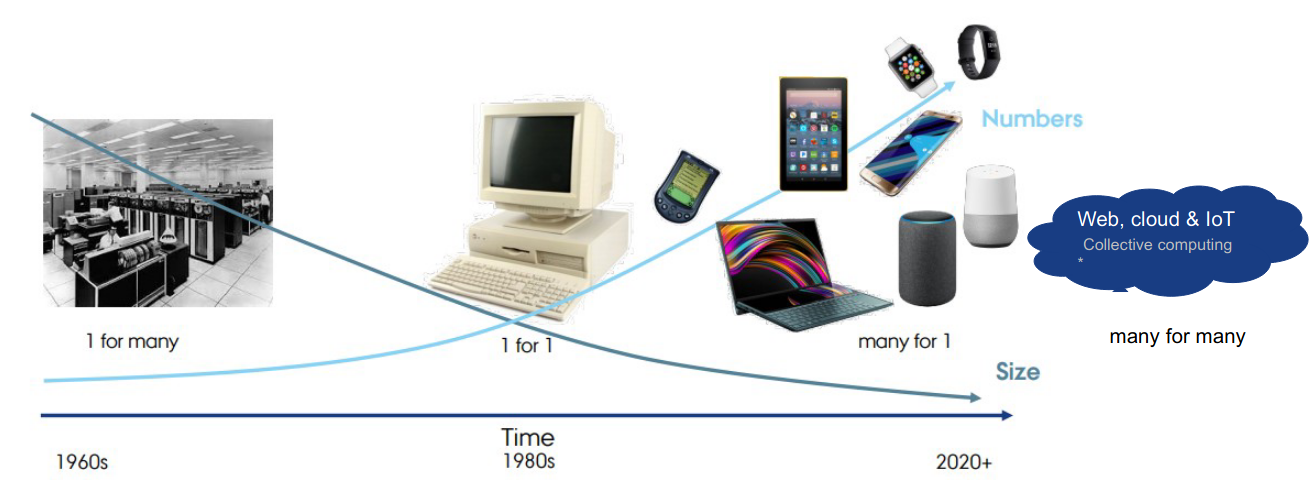
\includegraphics[width=\textwidth]{figs/three_computing_waves.png}
    \caption{The three (+ one expected) computing waves. Image: \cite{wagnerPervasiveComputing2022}. Theory: \cite{abowdWeiserUbiquitousCollective2016}}
  \end{figure}
\end{frame}

\begin{frame}
  \frametitle{Pervasive computing concepts}
  Important concepts\footnote{Selection based on slide from \cite{wagnerPervasiveComputing2022}}:
  \begin{enumerate}
    \item Calm technology
    \item Implicit HCI
    \item Context awareness
    \begin{itemize}
      \item Location awareness
    \end{itemize}
    \item Smart devices
    \item Smart spaces
  \end{enumerate}
  \note{
    Implicit HCI: When a user makes an action that is not explicitly aimed at a computer system but where the system understands it as an input. Could be opening a window or walking into a room.\\
    Context awareness: If we want our systems to truly be calm and help our users they must be aware of the current context. Could be whether a room is occupied or which mood the user is in.
  }

\end{frame}

\section{Methods}

\begin{frame}
  \frametitle{Prototyping}
  Sensor challenges:\footnote{Challenges paraphrased from \cite{wagnerContextAwareness2022}.}
  \begin{itemize}
    \item Which types of sensors do we need?
    \item How many are needed for the necessary fidelity?
    \item \alert{How are they perceived by the users?}
    \note{
      Project: Smart home environment. Used camera for emotion detection. Set the atmosphere in the room based on the emotional context.\\
      People were sceptical about our solution. People were especially sceptical towards the cameras as they are afraid that it is not secure.
    }
  \end{itemize}

  Prototyping: Systems engineering method for developing early iterations of a product.
\end{frame}

\begin{frame}
  \frametitle{Iterative prototyping}

    \begin{figure}
    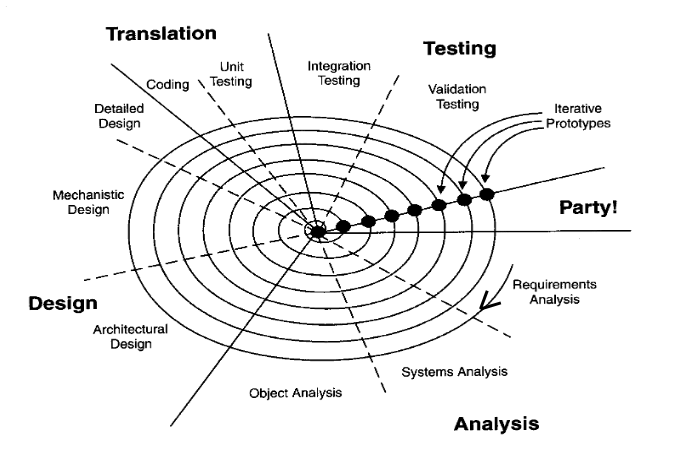
\includegraphics[width=0.9\textwidth]{figs/iterative_prototyping.png}
    \caption{Model for iterative prototyping. Image: \cite{wagnerPervasiveComputing2022}.}
  \end{figure}
  \note{
    The figure shows a model that was proposed by Stefan on how iterative prototyping can be done. \\
    In the context of pervasive systems, I would actually not follow necessarily follow this model strictly. Of course, this is all application dependent but in many cases, it may be beneficial to do some validation testing during or after the design phase to make sure that the end-user likes the idea. Otherwise, you risk ending up with a solution like ours, which we thought was very cool but the end-users hated.\\
    In our case, it could be concluded very early that the solution wasn't the best by simple pretotyping. The camera was central to our idea so we could collect some data as early as possible and disaffirm our idea. \textbf{Fail fast.}
  }
\end{frame}

\begin{frame}
  \frametitle{Context awareness}
  \begin{figure}
    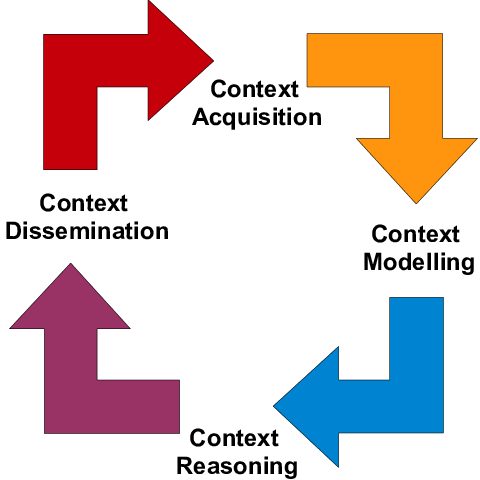
\includegraphics[width=0.5\textwidth]{figs/context_life_cycle_model.png}
    \caption{Context life cycle model. ''The simplest form of a context life cycle''. Quote and figure: \cite{pereraContextAwareComputing2013}}
  \end{figure}
  \note{
    The context life cycle model shows the minimum steps required in making a context-aware system. \\
    Acquisition: We acquire some sort of data from a sensor. Could be a light sensor. \\
    Modelling: We put it into the model that we built. Could be a linear regression in this case. \\ 
    Reasoning: We make a decision. The light should be off as the room is bright already. \\
    Dissemination: We act on the decision. Turn off the light if it is on or do nothing if it is off.
  }
\end{frame}

\section{Enabling Technologies}

\begin{frame}
  \frametitle{Pervasive Enabling Technologies}
  Pervasive enabling technologies \cite{wagnerPervasiveComputing2022}:

  \begin{itemize}
    \item Distributed systems
    \item Mobile technologies
    \item Sensors
    \item Novel interaction types
  \end{itemize} 
  \note{
    Distributed systems: Without being able to compute different parts across different nodes it would be impossible to make pervasive systems. In many cases, a pervasive system can be considered a distributed system.\\
    Mobile technologies: Often the entry point for a pervasive system is through a smartphone. More on this later. \\
    Sensors: The sensors are the ones providing data for the context model. It is a key technology in a pervasive system. \\
    Novel interaction types: For a true calm experience we need other means of interacting with the system than through phones and computer inputs. Speech, gestures and presence could be examples of this.
  }

\end{frame}

\begin{frame}
  \frametitle{Smart DEI Model}
  \begin{figure}
    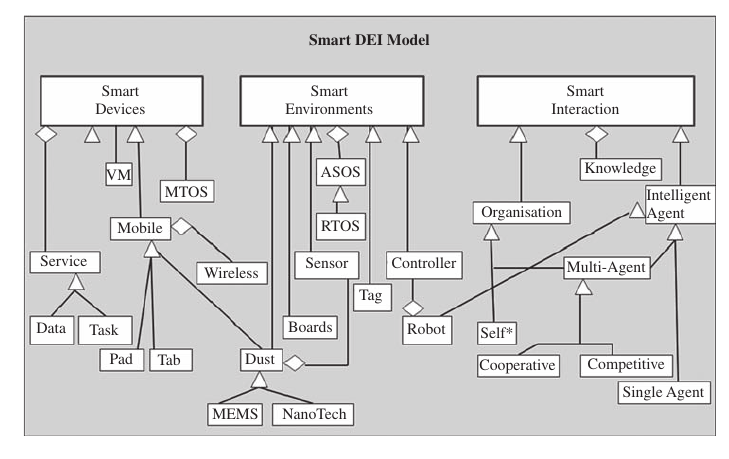
\includegraphics[width=0.9\textwidth]{figs/smart_dei.png}
    \caption{Smart DEI model describing pervasive enabling technologies. Triangles = subtypes. Diamonds = aggregations. \cite{posladUbiquitousComputingSmart2009}}
  \end{figure}
  \note{
    The figure shows various pervasive enabling technologies.
  }

\end{frame}

\section{Mobile Computing}

\begin{frame}
  \frametitle{Mobile Computing}
  Mobile computing:
  \vspace*{-1em}
  \begin{itemize}
    \item Main driver for pervasive systems
    \item Most pervasive systems rely in one way or another on an app\footnote{App not limited to a smartphone app. Could also be a smartwatch app.}
  \end{itemize}

  Limitations\footnote{Limitations paraphrased from \cite{wagnerPervasiveComputing2022}.}:
  \vspace*{-1em}
  \begin{itemize}
    \item You have to carry/wear them
    \item They need power - battery and processing
    \item Limited user interfaces - form factor and power
  \end{itemize}

  Can perhaps be replaced by: Ambient sensors, calm/novel interaction devices and collective technologies.
  \note{
    Typically a pervasive system can be interfaced through an app on one of our smart devices. \\
    Replaced: Ambient sensors could be PIR sensors or camera sensors. Calm interaction devices could be screens or audial devices. Collective technologies could be cloud computing - if the computations otherwise took place on the phone.
  }
\end{frame}

\begin{frame}
  \frametitle{Project}
  \begin{figure}
    \includegraphics[width=\textwidth]{figs/deployment_diagram.pdf}
    \caption{Deployment diagram of our project.}
  \end{figure}
\end{frame}

\section{References}
\begin{frame}[allowframebreaks]{References}
  \bibliographystyle{ieeetr}
  \bibliography{references}
\end{frame}
\end{document}
